\section{Manipulating deformable objects} \label{sec:lit_traditional}

% TOOD niet te veel herhalen 
This section provides important historical context and prior work in the rigid and deformable object manipulation literature. First, we discuss the traditional control approach to rigid object manipulation for robots and how these methods are challenging to generalize towards deformable object manipulation. Next, we provide a definition and categorization of deformable objects. For each category, we provide common tasks and solutions identified in literature.
% Finally, we highlight important work in the domain of robotic folding.

\subsection{Manipulating rigid objects}
Grasping and manipulation problems in robotics are traditionally solved by manually engineering subsystems for perception, planning and control \autocite{Siciliano2008}. A popular approach is using images as input observation to control the robot's motions. This approach is motivated by the advantage that images enable closed-loop control: non-contact and real-time measurements of the environment can be used to provide feedback to the motion trajectory of the robot. This principle is generally known as visual servoing \autocite{Hutchinson1996} and was first introduced in~\citeyear{Hill1979} by \textcite{Hill1979}. An archetypical pipeline consists of the following steps to grasp and manipulate an object \autocite{Corke1996}. First, observations such as images are used to estimate the state of the object. This state estimation stage usually executes pixel manipulations and image filtering in order to extract features. This object state is used to interpret the scene to calculate the relative position of the target object from the robot end-effector. Once the object is identified, it can be modelled to identify a suitable grasping point. Next, these grasping points are given to a motion planning system that calculates a trajectory to move the end-effector to the desired position and orientation. Finally, a low-level controller sends motor commands to the actuators to move the robot. An example of this archetype control pipeline is displayed in \cref{fig:canonical_robotic_manipulation_engineered_pipeline}.

\begin{figure}[p]
    \centering
    \subfile{figures/canonical-robotic-manipulation-pipeline/fig-canonical-robotic-manipulation-pipeline.tex}
    \vspace*{-10mm}
    \caption[Canonical engineered manipulation pipeline.]{\textbf{Canonical engineered manipulation pipeline with examples of each module.} Cameras record observations that are used to estimate the state of the cloth downstream. The modelling module calculates the deformations on the cloth if certain manipulations are executed. A planning module calculates the desired end-effector trajectory and sends the corresponding joint position to a low-level controller.
    }
    \label{fig:canonical_robotic_manipulation_engineered_pipeline}
\end{figure}

% Probleem met traditionele pipelines toepassen voor vervormbare objecten
Engineering modular, hand-tuned motor control pipelines have been successful for applications in manufacturing \autocite{Clocksin1985,Mochizuki1987}, car steering \autocite{Dickmanns1988}, robotic ping-pong \autocite{Andersson1987}, juggling \autocite{Rizzi1993} as well as fruit picking \autocite{Harrell1989}. However, all of these applications operate under the condition of rigid objects: the shape of the object will not change on contact.
When manipulating objects, this is of importance for determining stable grasping points. More concretely, restraining rigid objects relies on \textit{form closure} \autocite{Nguyen1988} or \textit{force closure} \autocite{Bicchi1995}: fully constraining relative motion of the object or having contact points that can counteract an external wrench through friction.
However, in the case of deformable objects, the object can deform during grasping and manipulation. This leads to exponentially higher dimensional configuration spaces compared to rigid object manipulation \autocite{Foresti2004}. For example, achieving form closure becomes impossible as it requires immobilizing every degree of freedom. Similarly, force closure becomes computationally intractable as it requires constantly incorporating the adapted shape of the object. For example, we visually show the deformations that occur when grasping a plastic cup versus a rigid glass when trying to achieve force closure. Furthermore, manipulation requires reasoning about the target shape of the object. These properties make many rigid object manipulation techniques hard to extend in the deformable object domain. Unfortunately, to date, the vast majority of robotic manipulation work deals with rigid objects whereas many objects are of deformable nature \autocite{Siciliano2008}.

\begin{figure}[htbp]
    \centering

    \begin{subfigure}[b]{0.95\textwidth}
        \centering
        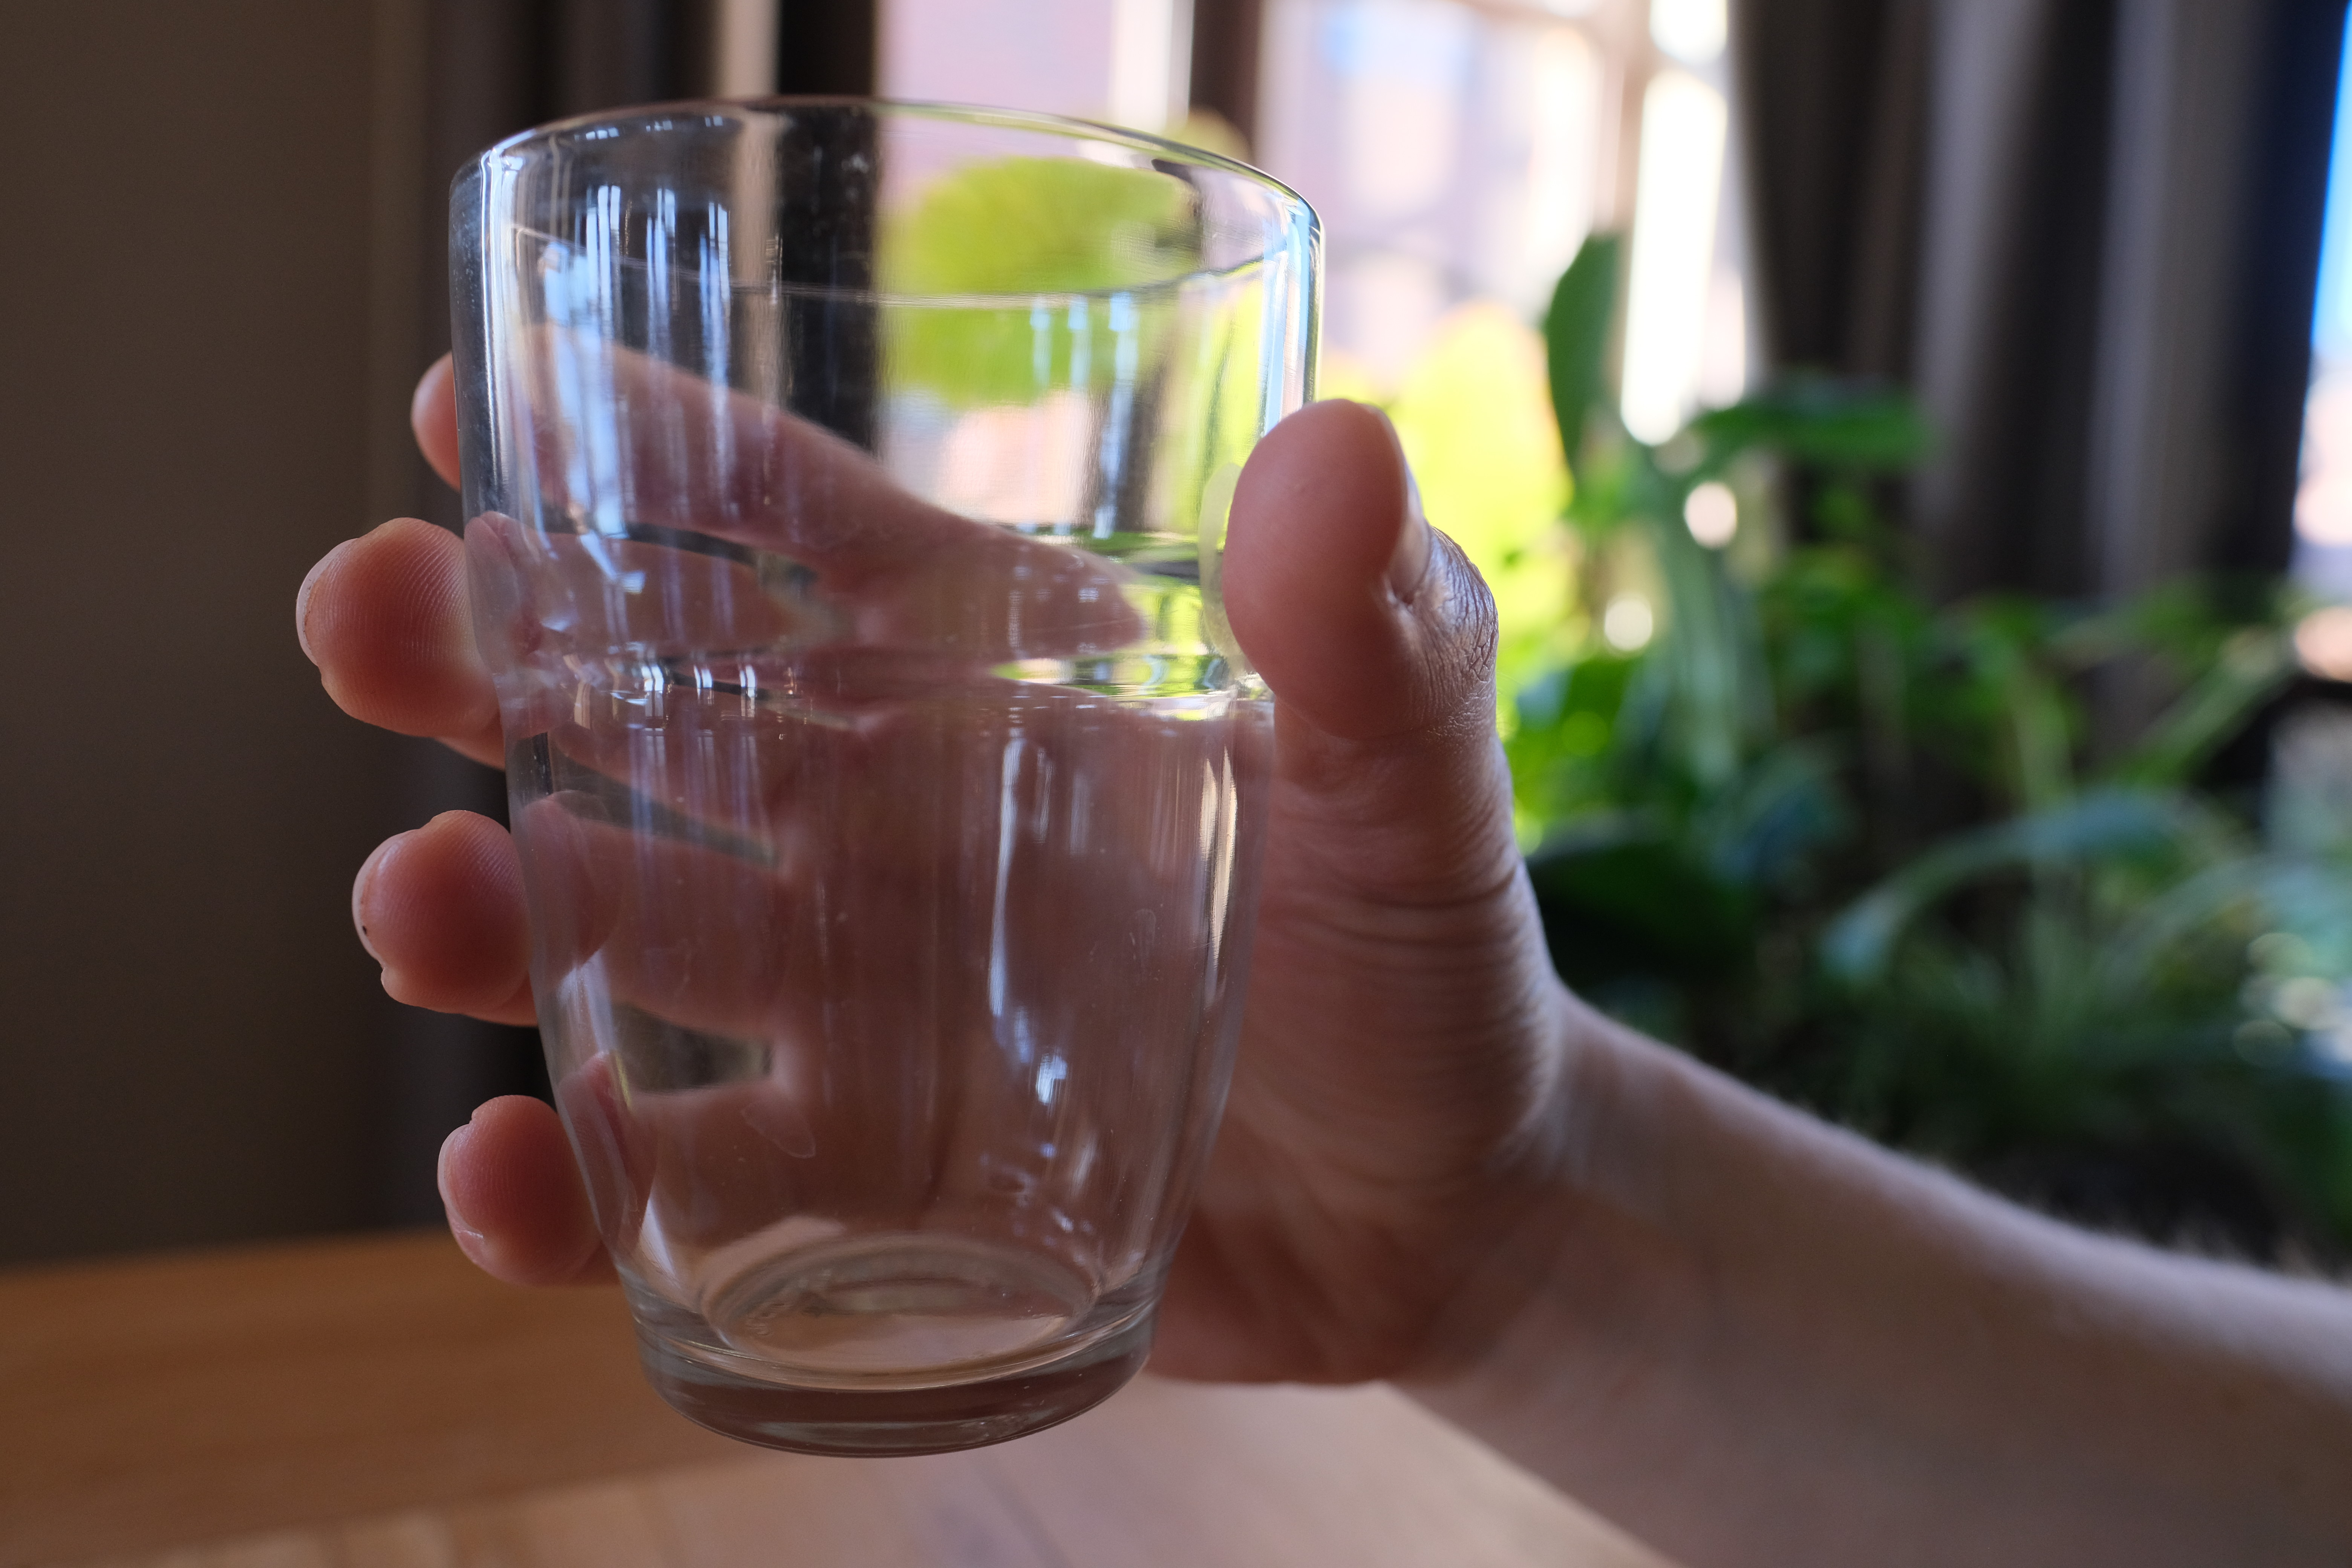
\includegraphics[keepaspectratio, width=\textwidth]{figures/fig_glass.jpg}
        \caption{}
        \label{fig:force_closure_deform_object_glass}
    \end{subfigure}
    % \hfill
    \begin{subfigure}[b]{0.95\textwidth}
        \centering
        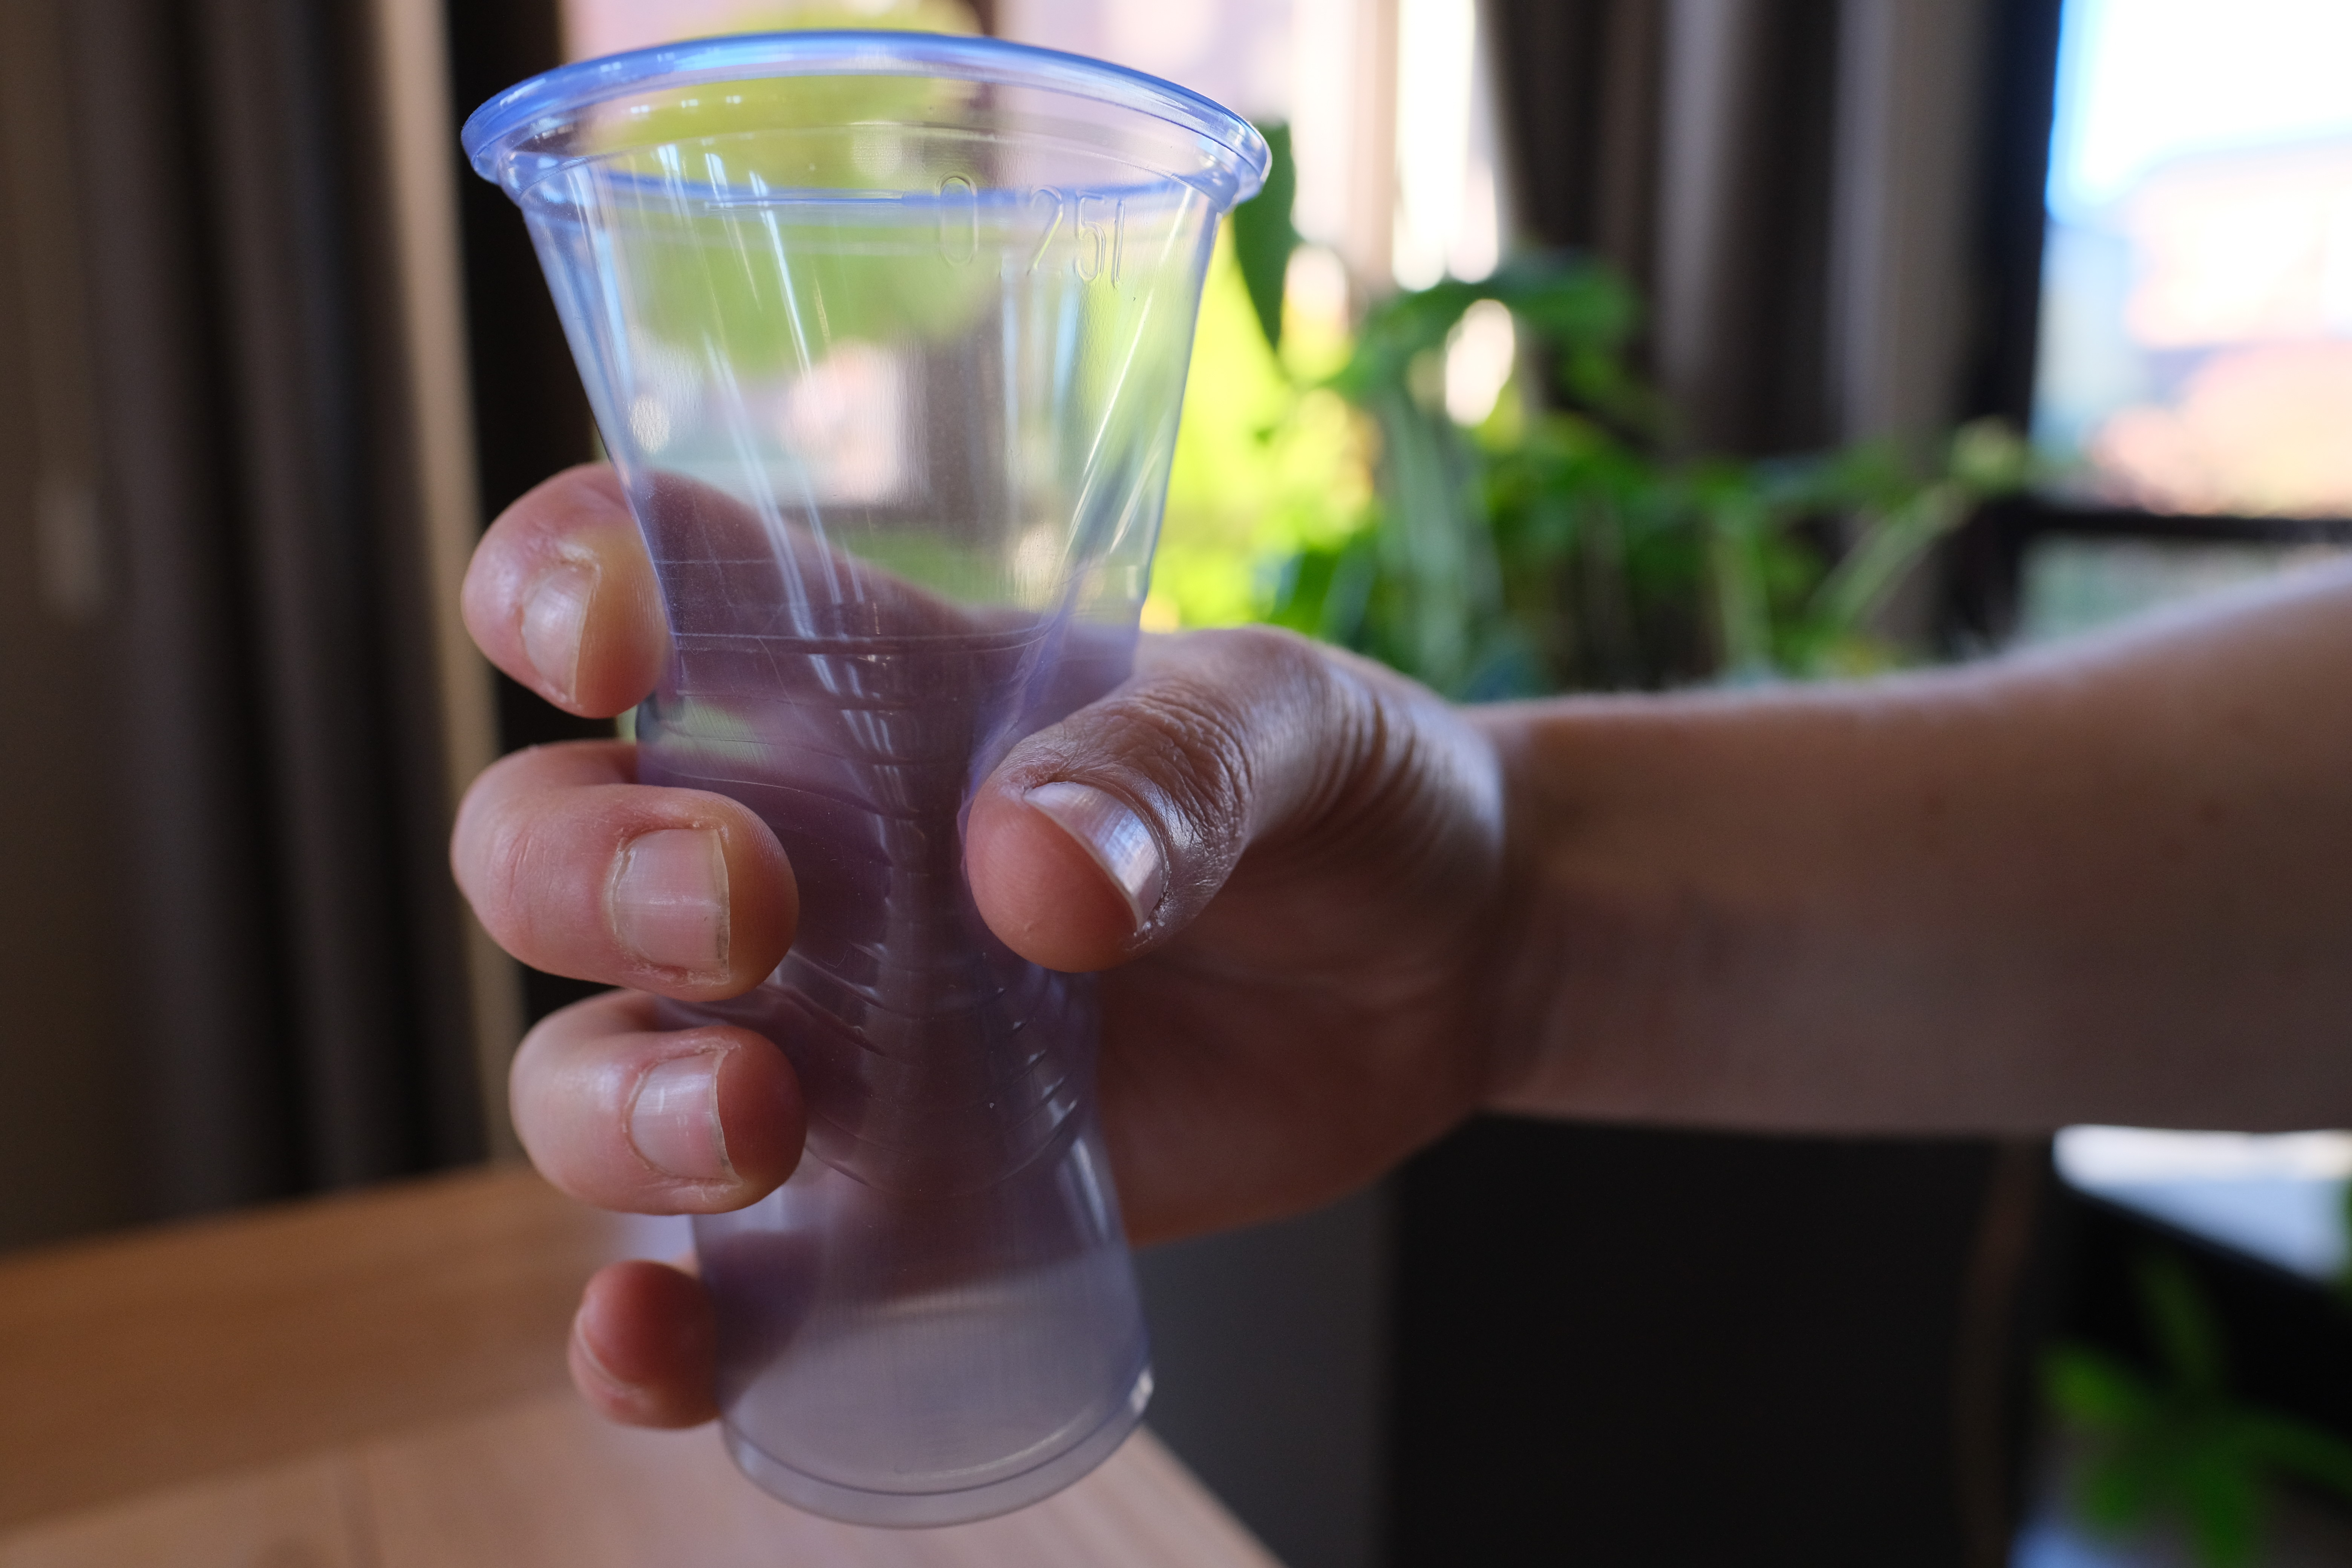
\includegraphics[keepaspectratio, width=\textwidth]{figures/fig_cup.JPG}
        \caption{}
        \label{fig:force_closure_deform_object_cup}
    \end{subfigure}

    \caption{Force closure on a rigid glass (a) and a deformable, plastic cup (b). The deformations of the plastic cup need to be taken into account when calculating a grasping pose.}
    \label{fig:force_closure_deform_object}
\end{figure}

\subsection{Deformable objects: definition, categorization, tasks and solutions}
% Vervormbare objecten: wat zijn ze, categorisatie, welke taken en welke oude pipelines bestaan er
A deformable object is an object whose shape changes when being subject to an external force. This deformation can be temporary and reversible (\textit{elastic}), permanent (\textit{plastic}) or a combination of both (\textit{elasto-plastic}). Deformable objects are found in industrial settings, agriculture and household items. A common categorization \autocite{Saadat2002,Jimenez2012} is based on the geometry of the object: how many dimensions are significantly larger than the other dimensions. Note that this is different to other categorizations such as categorizing based dimensionality of the object itself instead of its deformable dimensions.
\keyWithTitle{Deformable objects}{A deformable object is an object whose shape changes on interaction and can be categorized based on the number of dimensions negligible for manipulation planning.}
In its simplest setting, the deformable object is one dimensional: ropes, strings, cables, threads and catheters, among others. Some of these examples are shown in \cref{fig:dlo_examples}. These objects are also known as deformable linear objects. The term \textit{linear} refers to one dimension being dominant over the other two dimensions. Common tasks for deformable linear objects involve grasping and manipulating ropes, for example, knot tying. Early motor control architectures for solving tasks regarding deformable linear objects used either an open-loop approach or simple visual servoing to execute the motion. An early work clearly demonstrating modular control pipelines is the project of~\citeauthor{Inaba1987} in~\citeyear{Inaba1987}. Their method employs visual servoing for manipulating a rope into a ring and then tying the rope. 
Their perception module uses stereo images to detect the rope and the ring. The planning module is hard-coded to iterate through a set of predefined steps while using the detected centre of the ring and 3D coordinates of the endpoints of the rope from the perception module. An inverse kinematics module provides a target trajectory to the low-level controller. Similar modular pipelines can be found in \autocite{Remde1999} for grasping a rope and in \autocite{Saha2007} where knots are tied with needles using probabilistic trajectories of the rope from a simulated model. Incorporating motion primitives, i.e.\ a predefined set of motor actions corresponding to high-level actions, in the planning module is used in \autocite{Yamakawa2008, Vinh2012} to tie knots in a rope.

\begin{figure}[htbp!]
    \centering
    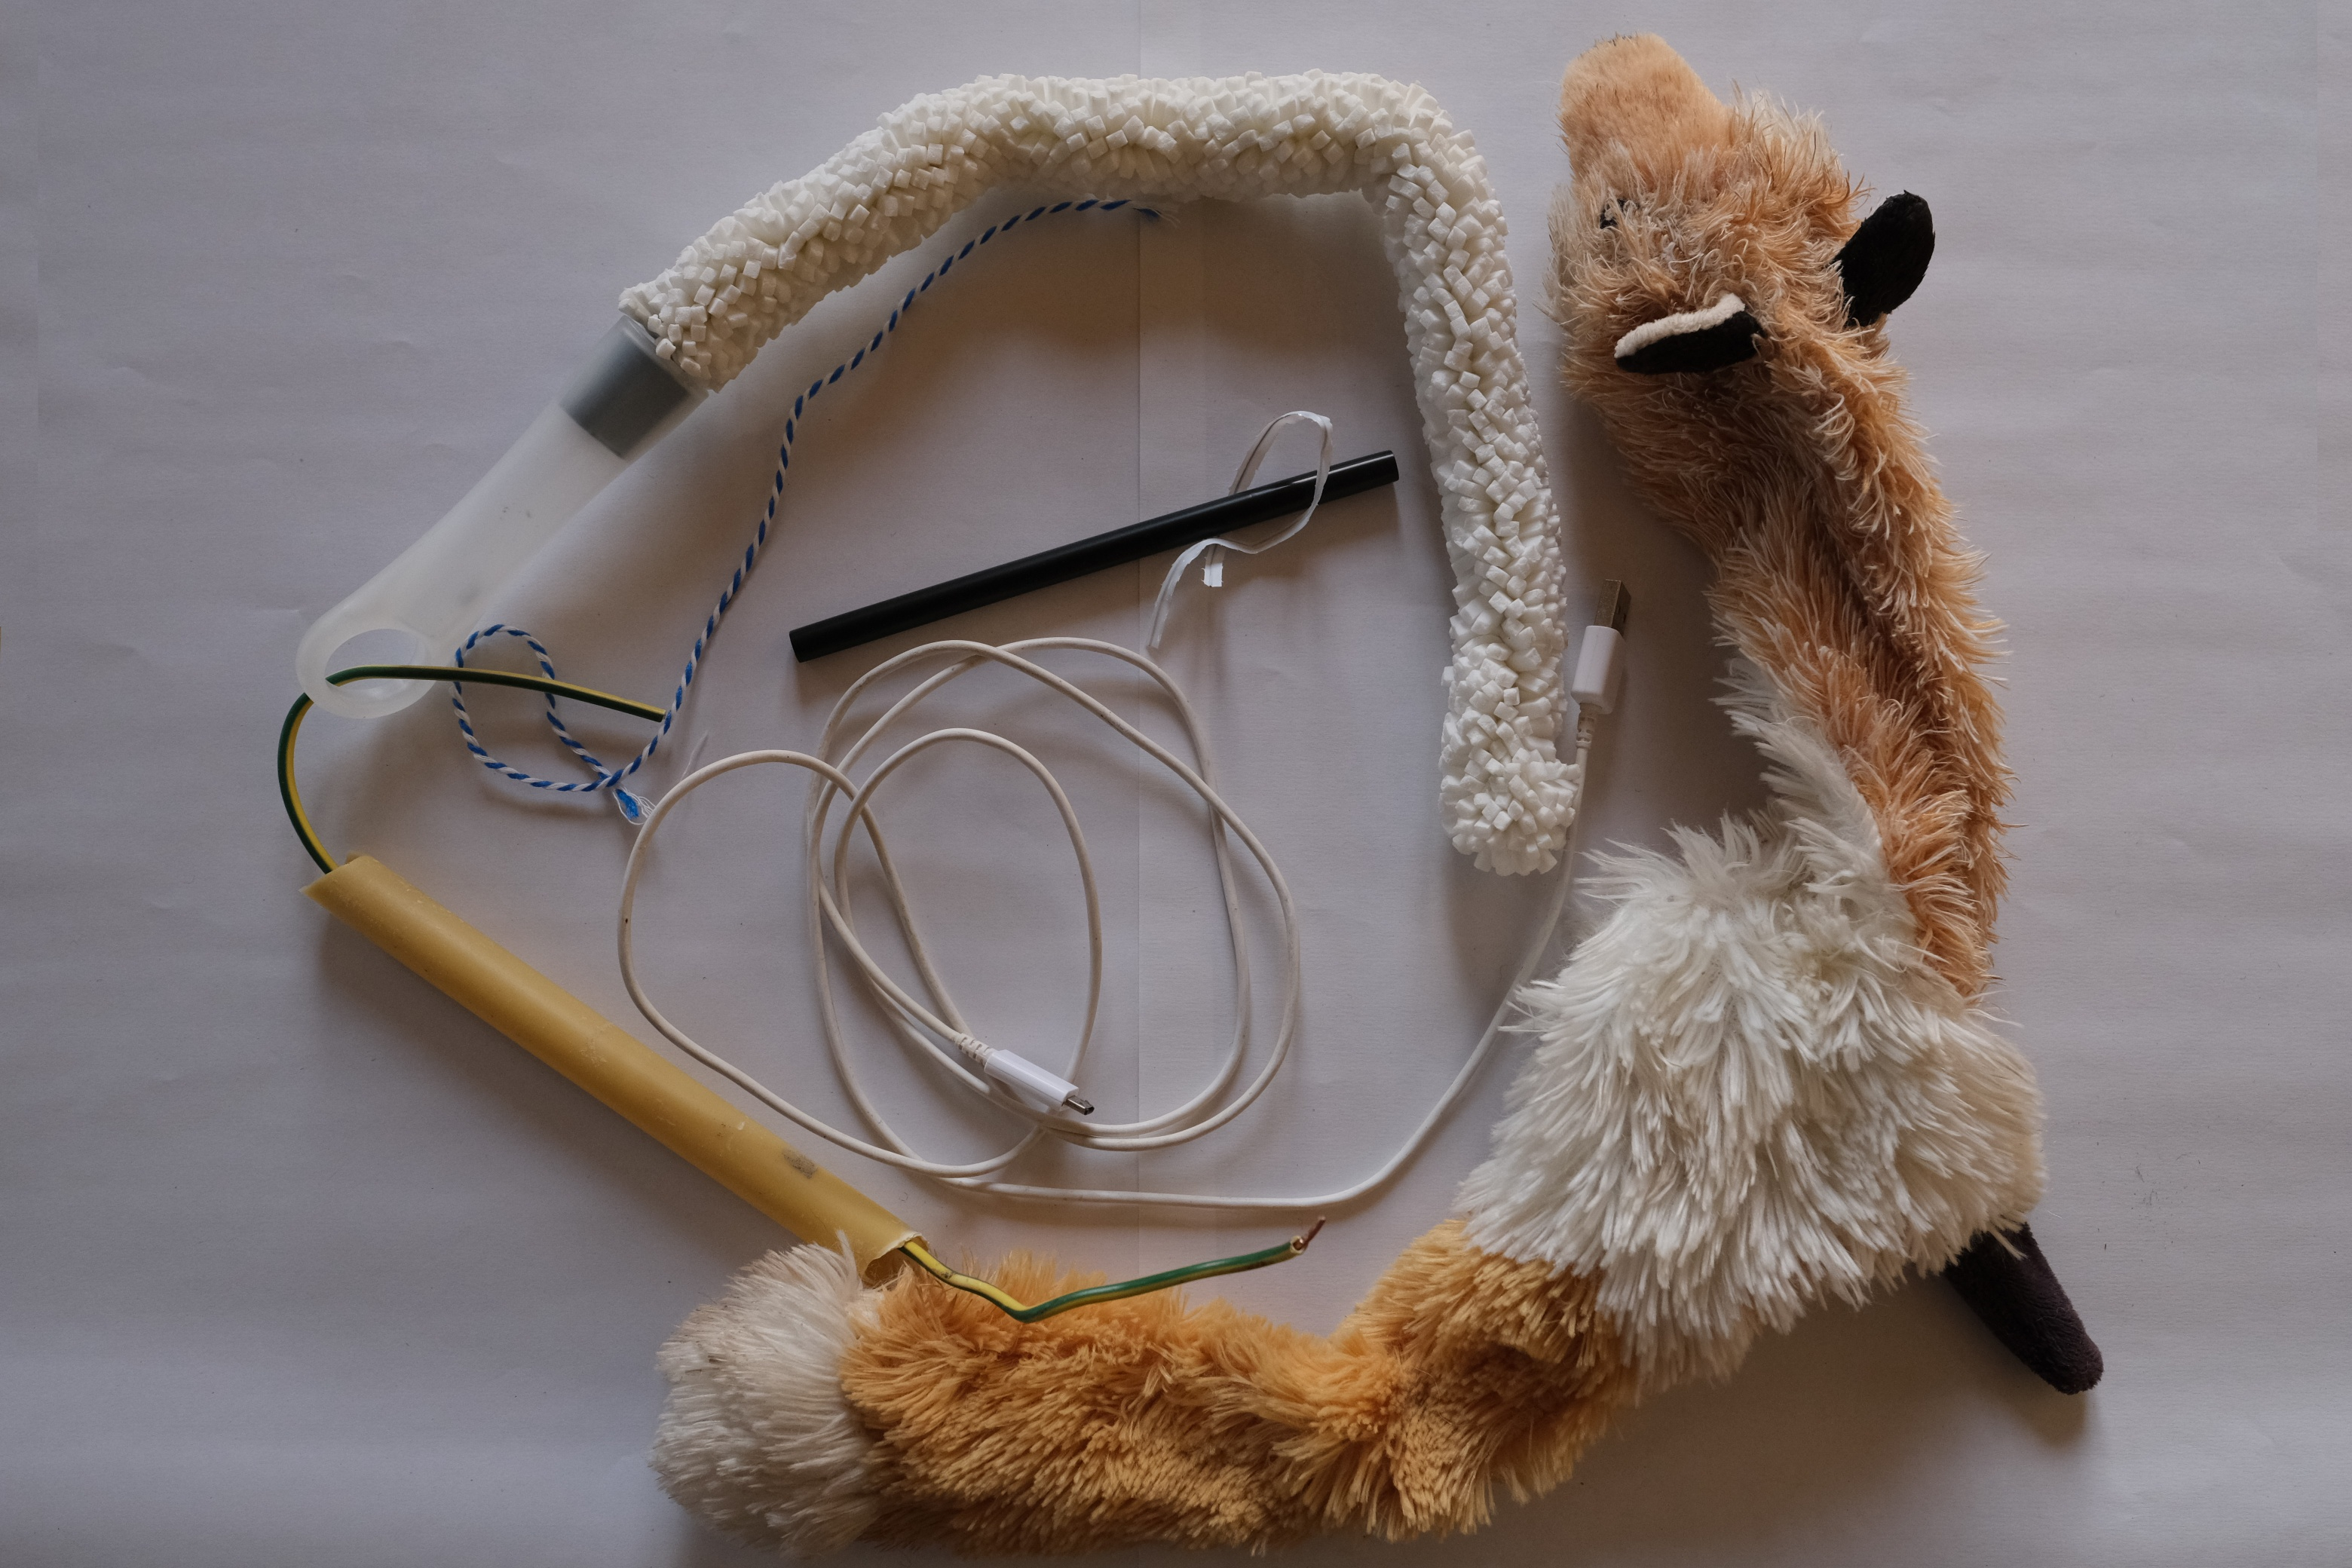
\includegraphics[keepaspectratio,width=\textwidth]{figures/fig_dlos.JPG}
    \caption{Examples of deformable linear objects and an application of putting an electrical wire into a rigid pipe.}
    \label{fig:dlo_examples}
\end{figure}

% 2D objects klassieke pipelines
Deformable \textit{linear} objects become deformable \textit{planar} objects when two dimensions are significantly larger than the third dimension. 
In this case, the planning module can disregard the thickness of the material for manipulation. Canonical examples are given in \cref{fig:planar_deform_objects_examples} and contain objects such as clothing, thin-shelled objects like plastic bottles, fabric, paper, and plastic bags, deformable sheets, cards and foam materials. A classic example of paper folding is robotic origami, in which a robot has to sculpt a piece of paper into the desired shape by folding. This problem was tackled with an open-loop control architecture in \autocite{Balkcom2008} to produce a folded hat. \Textcite{Elbrechter2012} takes this a step further by using vision, simulation and fiducial markers on the paper to grasp and fold a paper with a five-fingered end-effector. Related to origami is carton folding and metal sheet bending. Typical control strategies \autocite{Liang1999,Liu2003,Aomura2002} consist of finding the correct locations and sequence of bending operations by modelling the object as a collection of panes articulated through hinge joints. Robotic manipulation of bags has been less studied due to the complexity of modelling and manipulating bags. To circumvent this complexity, dedicated hardware has been researched for grasping \autocite{Kazerooni2005} and unloading \autocite{Kirchheim2008} sacks. A general-purpose two-fingered robotic gripper is used in \autocite{Klingbeil2011} to grasp objects from a table, search the barcode and drop the object into a bag. The planner uses 3D points clouds of depth images taken by a camera. However, they assume the bag is already open for insertion and do not consider any possible deformations caused by touching or dropping an item into the bag.

In the context of this research, it is of interest to note that garments satisfy the same geometrical property of having one negligible dimension as objects such as paper and plastic bottles. However, the main characteristic distinguishing cloth is the compression strength: compared to other two-dimensional deformable objects, cloth does not possess any significant compression strength. Given that the current work deals with manipulations of clothing items, we dedicate \cref{sec:lit_cloth_folding_pipelines} to elaborate on cloth manipulation pipelines.

\begin{figure}[htbp!]
    \centering
    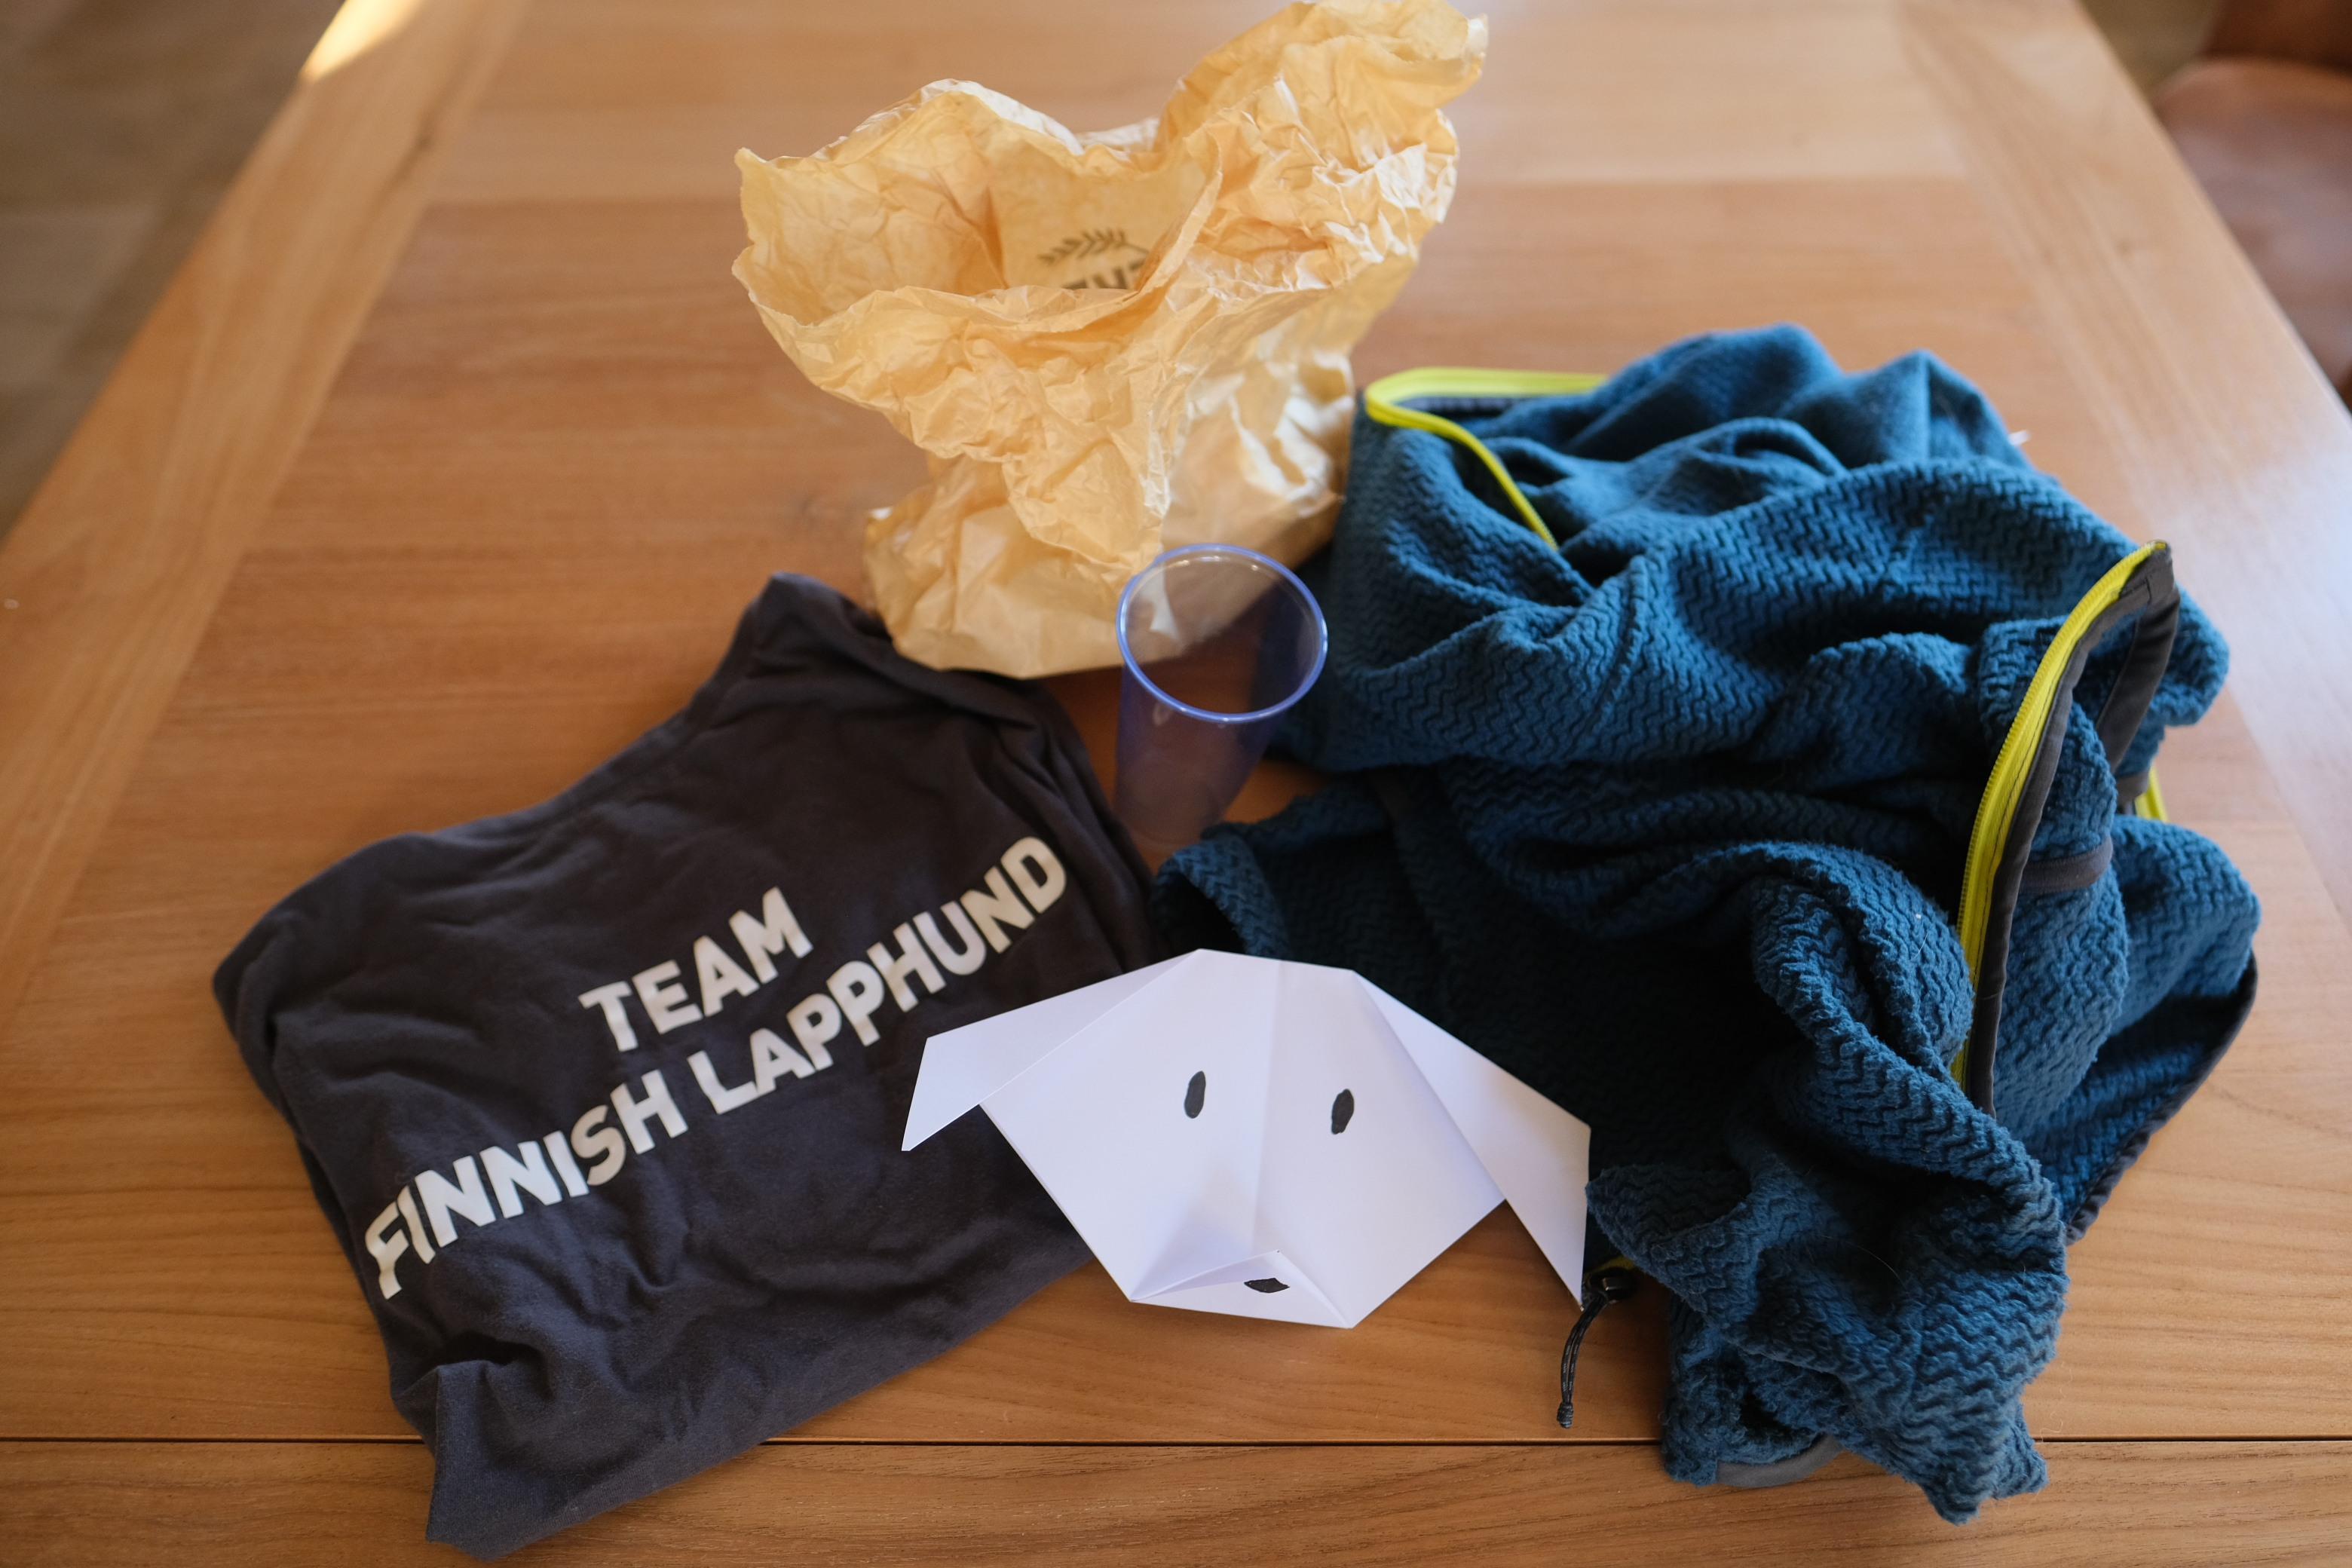
\includegraphics[keepaspectratio,width=\textwidth]{figures/fig_2d_deformables_ex.JPG}
    \caption{Examples of 2D deformable objects: origami, paper bag, shirt, jumper and a cup.}
    \label{fig:planar_deform_objects_examples}
\end{figure}

% 3D objects klassieke pipelines
The final category of deformable objects is \textit{volumetric deformable objects} whose deformations across all dimensions of the object are of relevance. Some examples are shown in \cref{fig:volumetric_deform_objects_examples}. These are objects such as food, plush toys and sponges. In the case of food products, deformations can be caused by both grasping and processing operations such as slicing. In general, 3D deformable objects are the least researched type of deformable objects \autocite{Sanchez2018}. An exception to this is soft tissue, which is important for medical application. We refer the reader to the review paper by \textcite{Taylor2016} for an overview of medical robots in surgery applications. For an overview of robotic manipulation of food products, we refer to the survey by \textcite{Chua2003}.

\begin{figure}[htbp!]
    \centering
    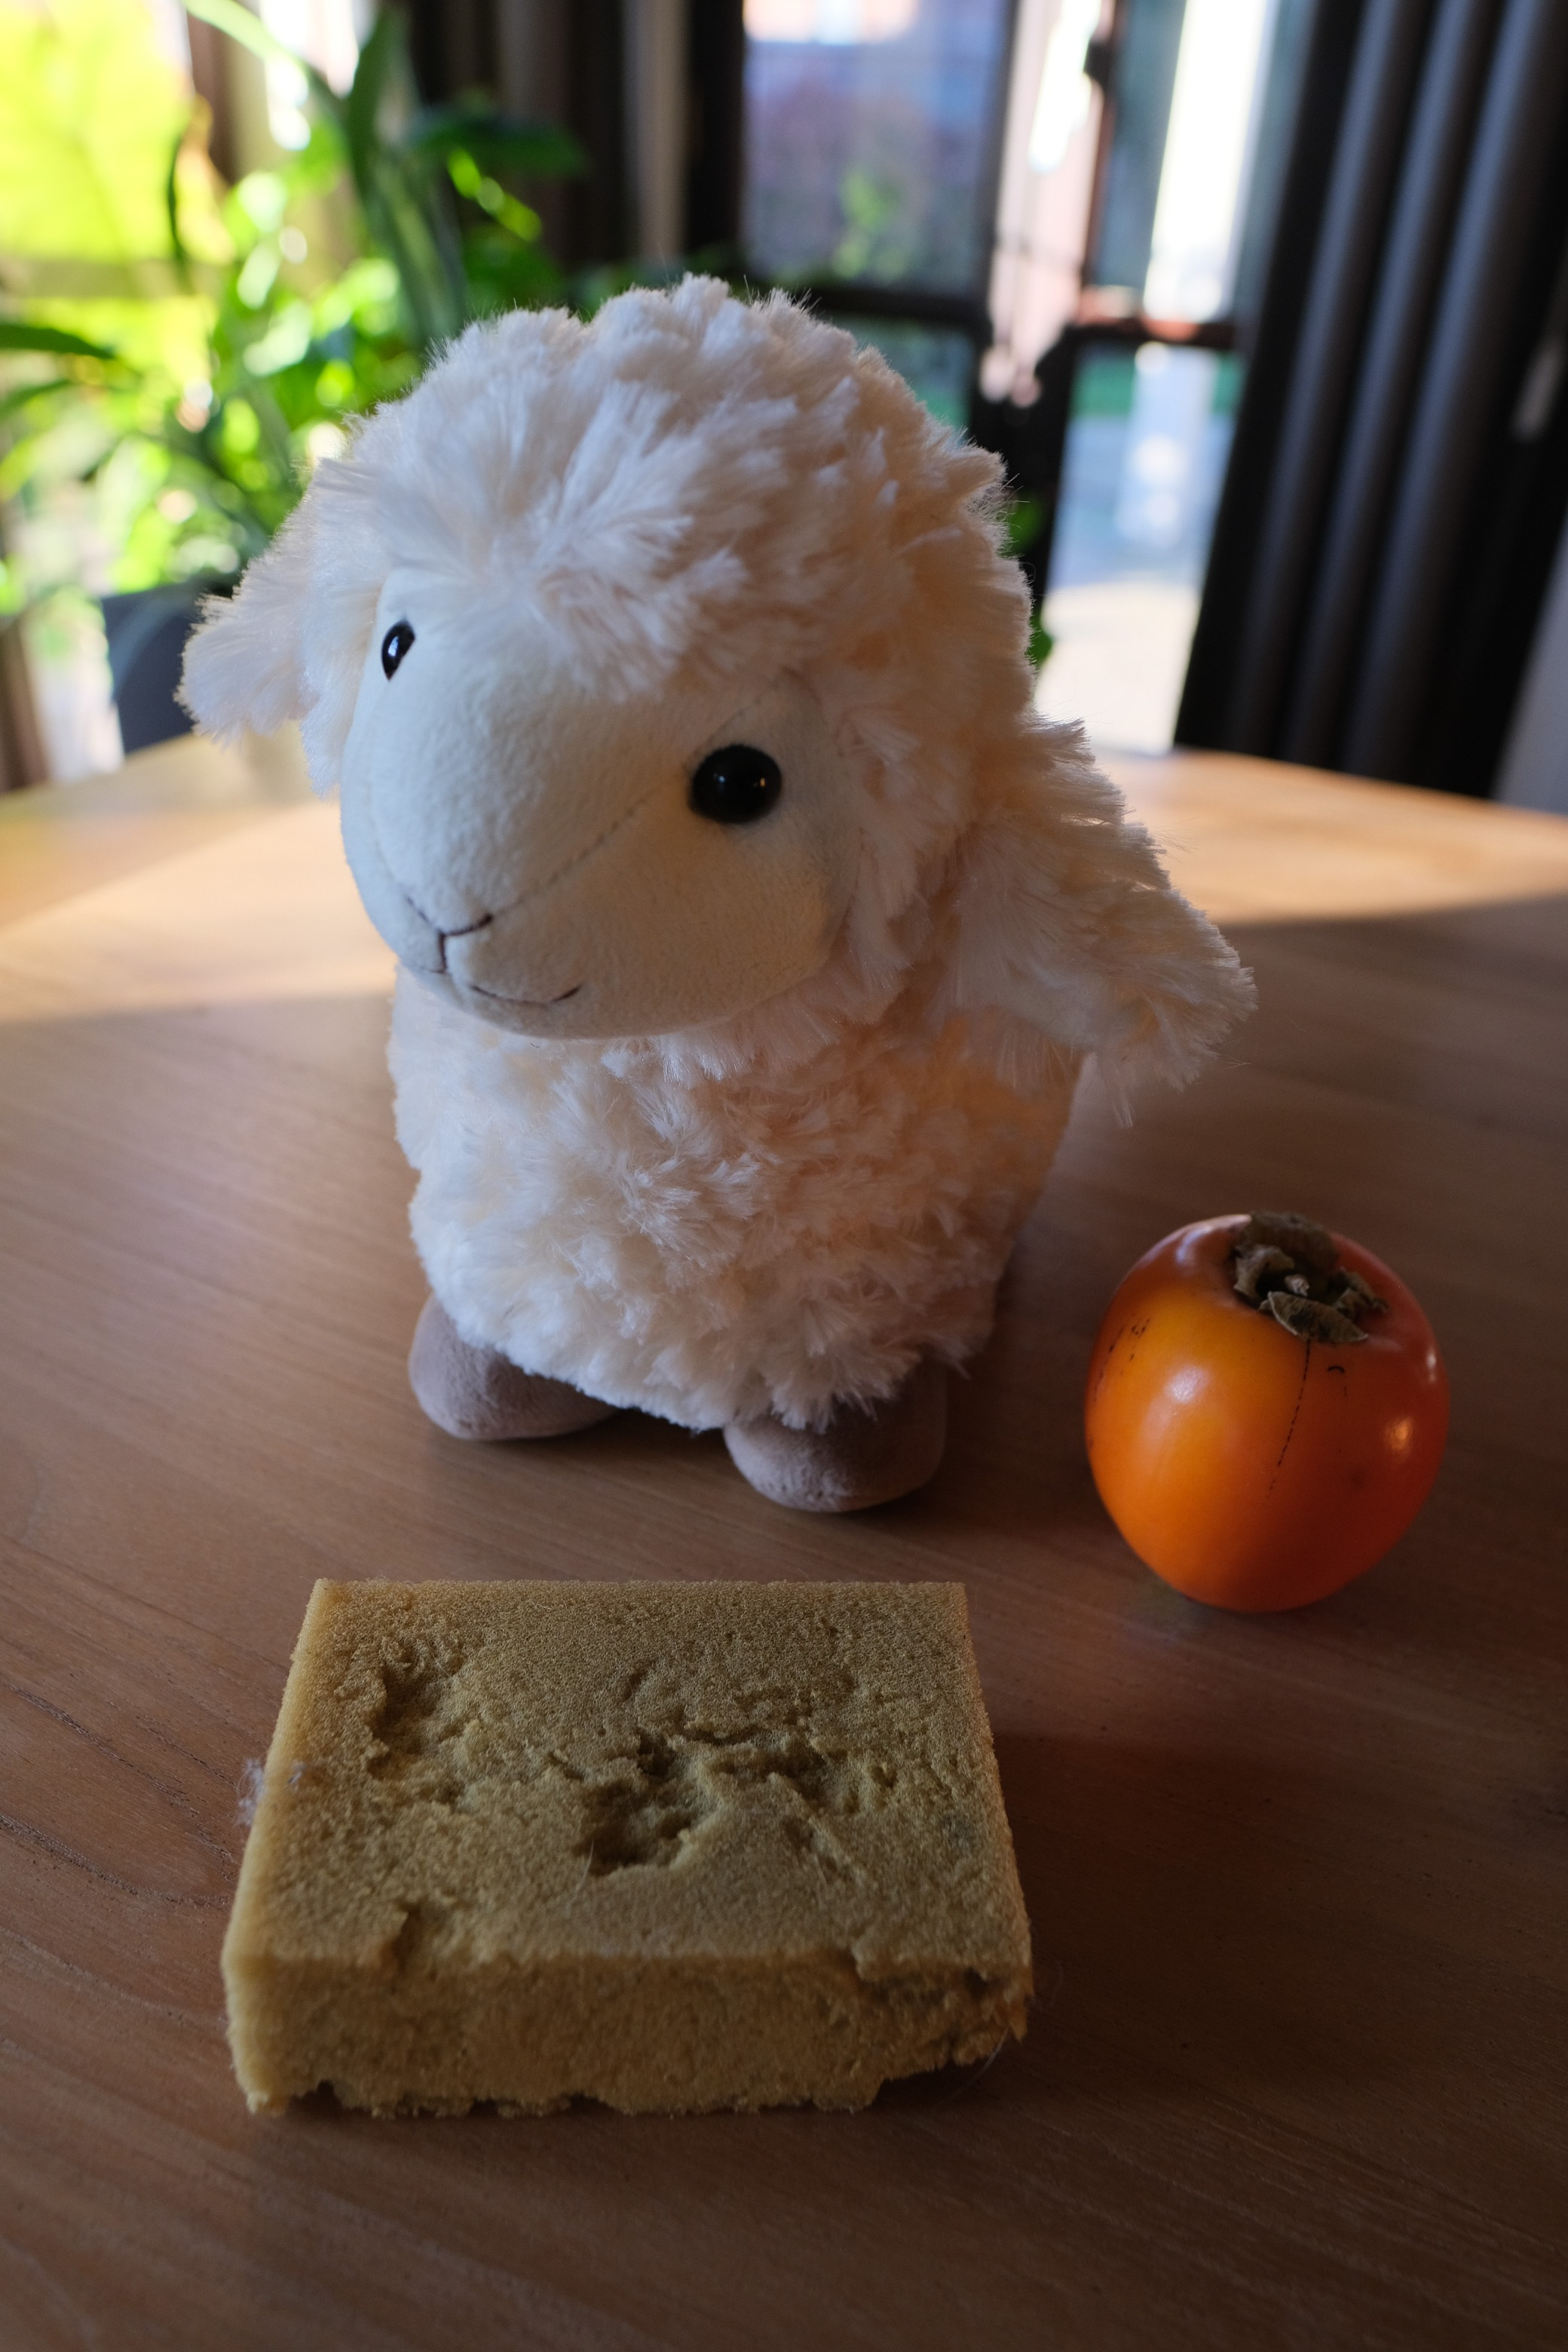
\includegraphics[keepaspectratio,width=\textwidth]{figures/fig_3d_deformables_ex.JPG}
    \caption[Solid deformable objects]{Examples of volumetric deformable objects: sponge, fruit and plush toy}
    \label{fig:volumetric_deform_objects_examples}
\end{figure}